\section{The Lipkin model}

First we show that our implementation of the restricted Boltzmann machine manages to converge towards the ground state energy. With a system size of $25$ particles we get the convergence:

\begin{figure}[H]
  \begin{center}
    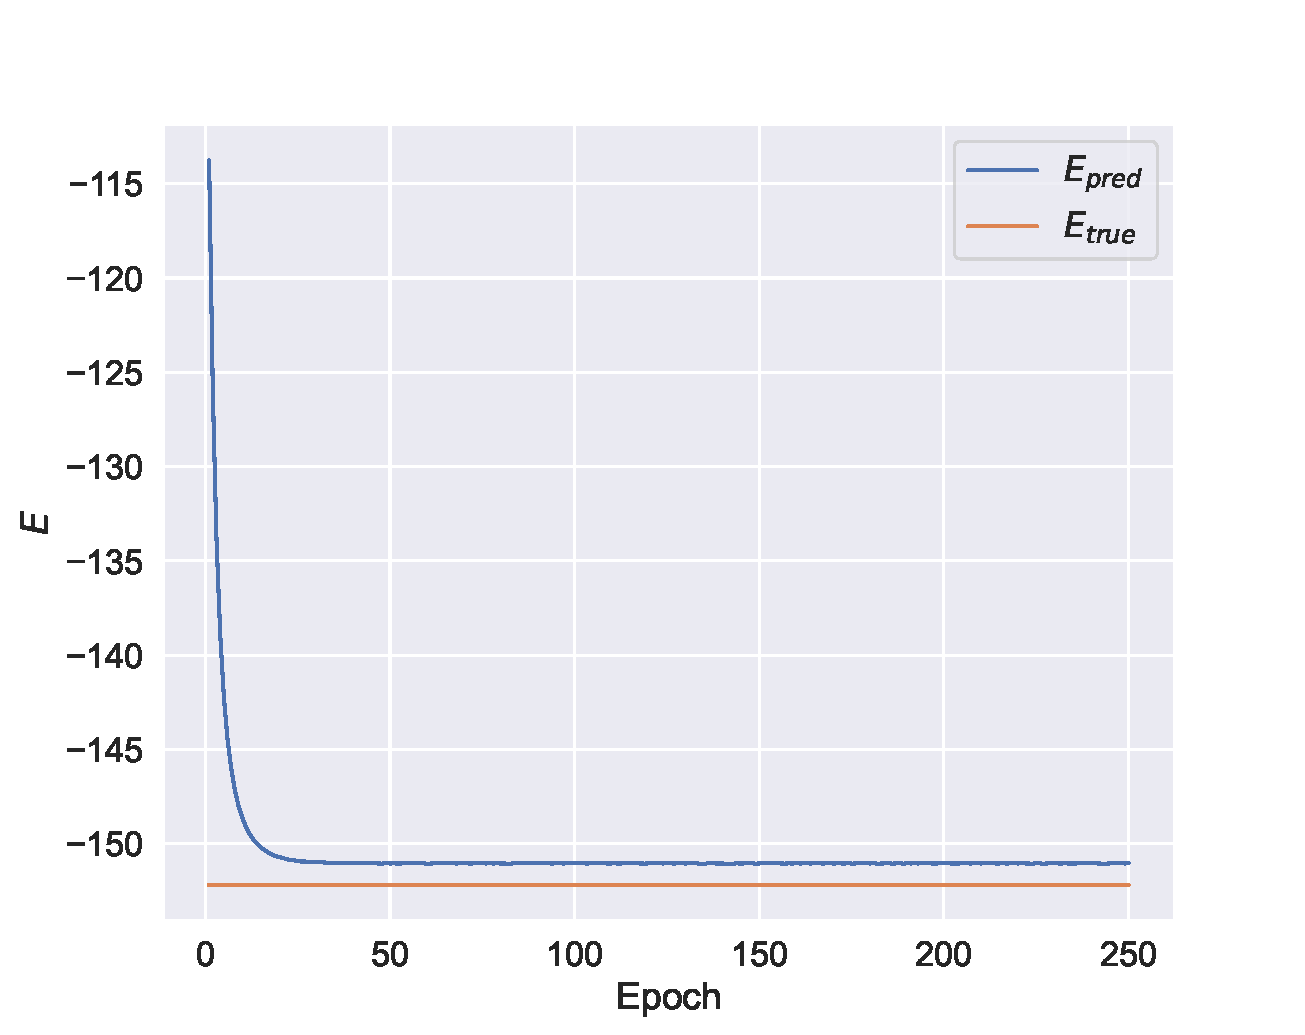
\includegraphics[width=0.95\textwidth]{Figures/Plots/Lipkin/Result25conv.pdf}
  \end{center}
  \caption{The convergence of the predicted ground state energy for the Lipkin model with $25$ particles, $\varepsilon = 2$, $V = -1$ and $W=0$.}\label{fig:res25conv}
\end{figure}

Where the final predicted energy is $E_{rbm} = -151.0 \pm 8.8$. The RBM converge towards a value that is slightly above the true value, and this is seemingly the closest the RBM manages to get. If we look at the gradients for the visual and hidden bias we see that they approach zero:

\begin{figure}[H]
  \begin{center}
    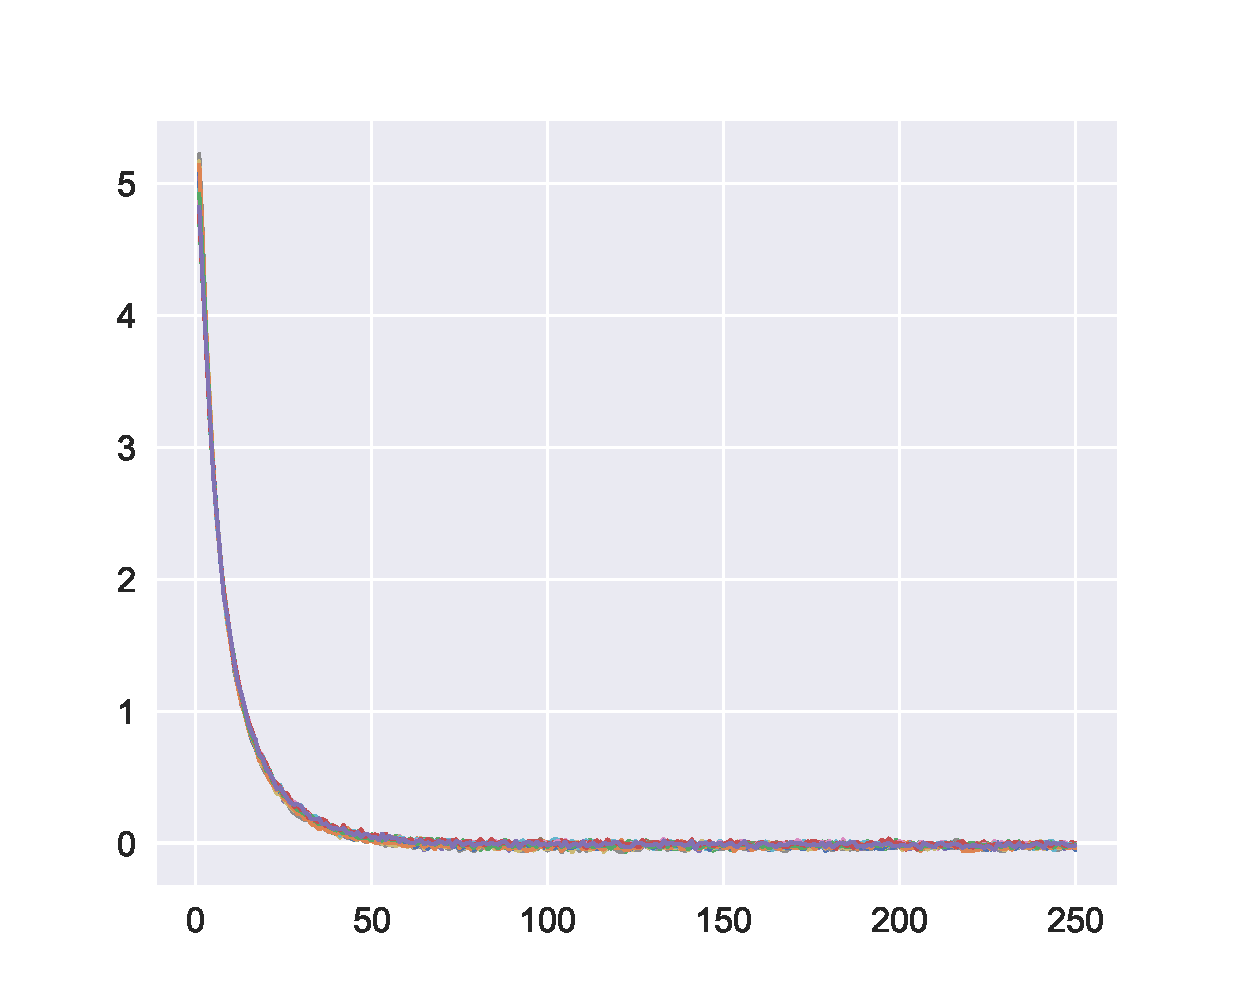
\includegraphics[width=0.95\textwidth]{Figures/Plots/Lipkin/Result25dvb}
  \end{center}
  \caption{The convergence of the gradient with respect to the visual layer bias. Lipkin model with $25$ particles, $\varepsilon = 2$, $V = -1$ and $W=0$.}
\end{figure}

\begin{figure}[H]
  \begin{center}
    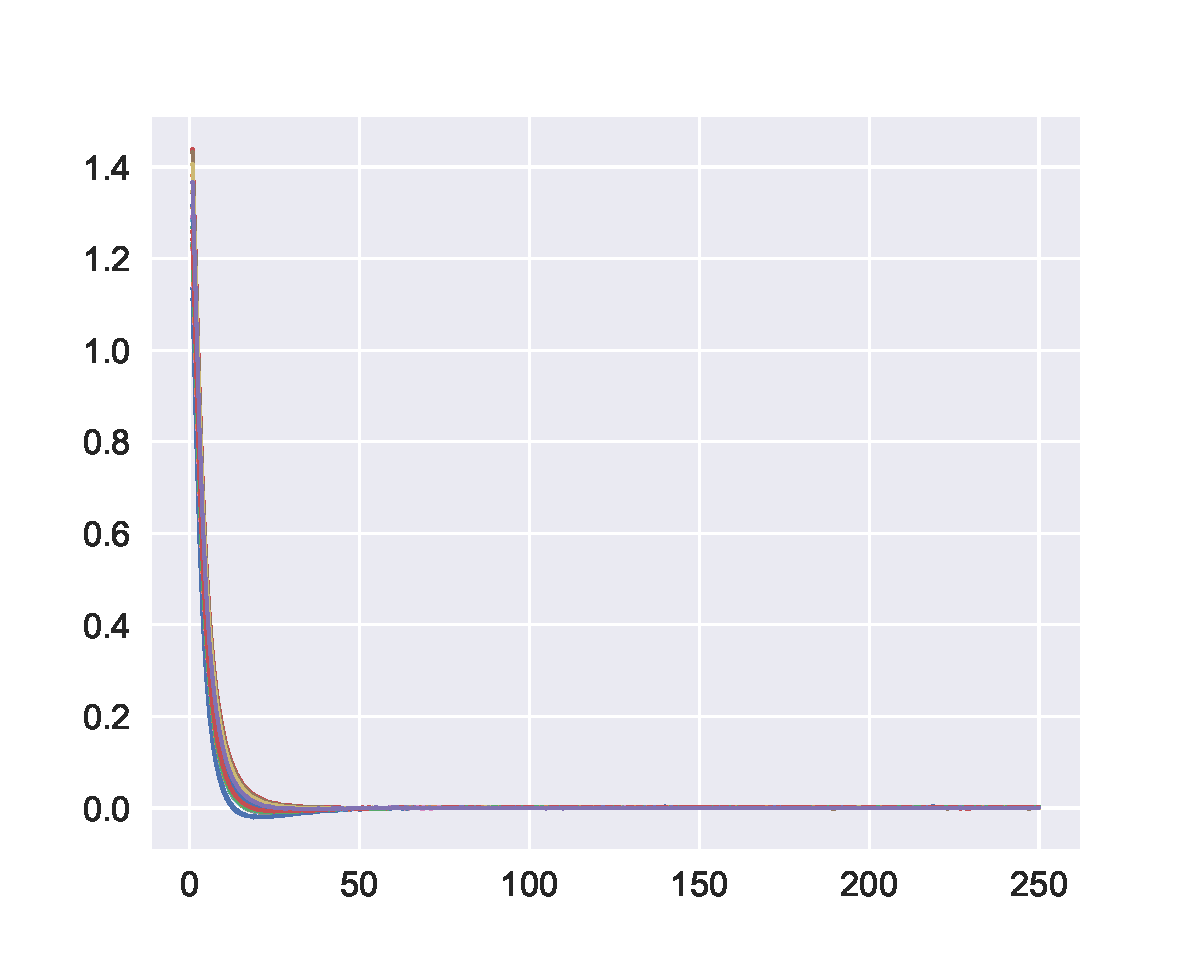
\includegraphics[width=0.95\textwidth]{Figures/Plots/Lipkin/Result25dhb}
  \end{center}
  \caption{The convergence of the gradient with respect to the hidden layer bias. Lipkin model with $25$ particles, $\varepsilon = 2$, $V = -1$ and $W=0$. As there are twenty five of the dimensionless variables we have refrained from adding a legend.}
\end{figure}

This means that the RBM has found its solution with the most even local energy between its samples, but it is important to remember that the $\psi_{rbm}$ is not the exact wavefunction, and since we have

$$E_{rbm} \geq E_0 \; ,$$

the machines best approximation of it has a higher energy in \ref{fig:res25conv}.

\subsection{The effect of \texorpdfstring{$\varepsilon$}{epsilon} on RBM prediction accuracy}

To look at the effect $\varepsilon$ has on the RBM's accuracy we first look at the machines prediction for no interaction strength, $V=0$ and $W=0$. For a small Lipkin model with $16$ particles we see the variance evolve as follows:

\begin{figure}[H]
  \begin{center}
    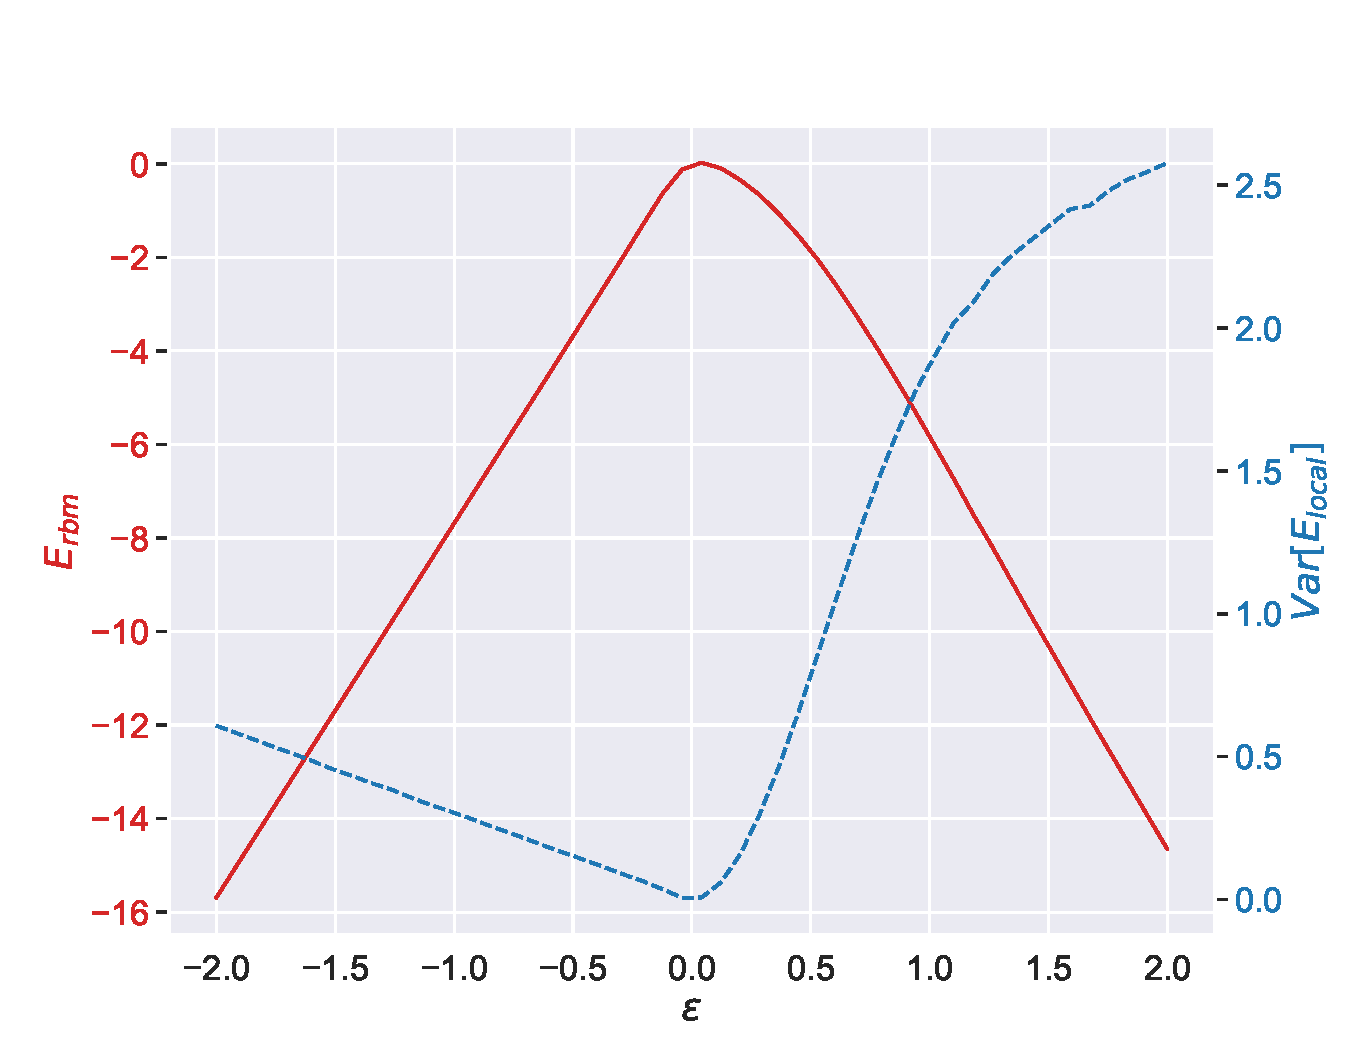
\includegraphics[width=0.95\textwidth]{Figures/Plots/Lipkin/[eps][-2.0-2.0][e=500][n=16][V=0][W=0]}
  \end{center}
  \caption{The RBM prediction of the ground state energy for the $16$-particle Lipkin system with $V=0$ and $W=0$.}
\end{figure}

We see that the RBM's accuracy improves towards $\varepsilon=0$, which is not that surprising, as at $\varepsilon = 0$ all wavefunctions gives the correct ground state energy of $E_0 = 0$. Aside from that we see a asymmetry between the variance for $\varepsilon = -2$ compared to $\varepsilon = 2$. As the ground state energy increases with higher $\varepsilon$ it is intuitive that the variance increases as well, because the differences between the machine state and the true wavefunction has higher impact on the local energies. The development of the variance above would indicate that the RBM has an easier time aligning all particles with spin up than spin down. 

The RBM manages to come very close to the exact wavefunction for all $\varepsilon$ and the reason for this is most likely the fact that the exact wavefunction for the ground state consist of only one basis state. This makes it easy for the machine to approximate by the fact that it is not limited by accuracy, it can get the distribution to be exactly $p(\ket{\psi}) = 1$ for the correct basis state $\ket{\psi}$ and get the others exactly to zero. Another driving factor for the accuracy of the simple case of no interaction strength may be that any divergence from the approaching the single-basis-state wavefunction has a increase in variance. As a reminder, we have the machine state:

$$\psi_{rbm} = \alpha_1\ket{\psi_1} + \alpha_2\ket{\psi_2} + \dots \alpha_n\ket{\psi_n} \; ,$$

and the true ground state wavefunction

$$\psi_{true} = \beta_1\ket{\psi_1} + \beta_2\ket{\psi_2} + \dots \beta_n\ket{\psi_n} \; .$$

For the non-interactive case one coefficient $\beta$ is one and the rest are zero. A wavefunction which consist of several basis states, where more than one $\beta$ is greater than zero, we could call a more diverse wavefunction. When the RBM would approach a diverse wavefunction a change in one of the coefficients $\alpha$ would affect the local energy of all basis state, where some would increase and some would decrease. For the non-interactive model, any such change would only result in an increase of local energy unless it is of the single basis state that the true wavefunction consists off. This stays the same for Lipkin models with more particles as well:

\begin{figure}[H]
  \begin{center}
    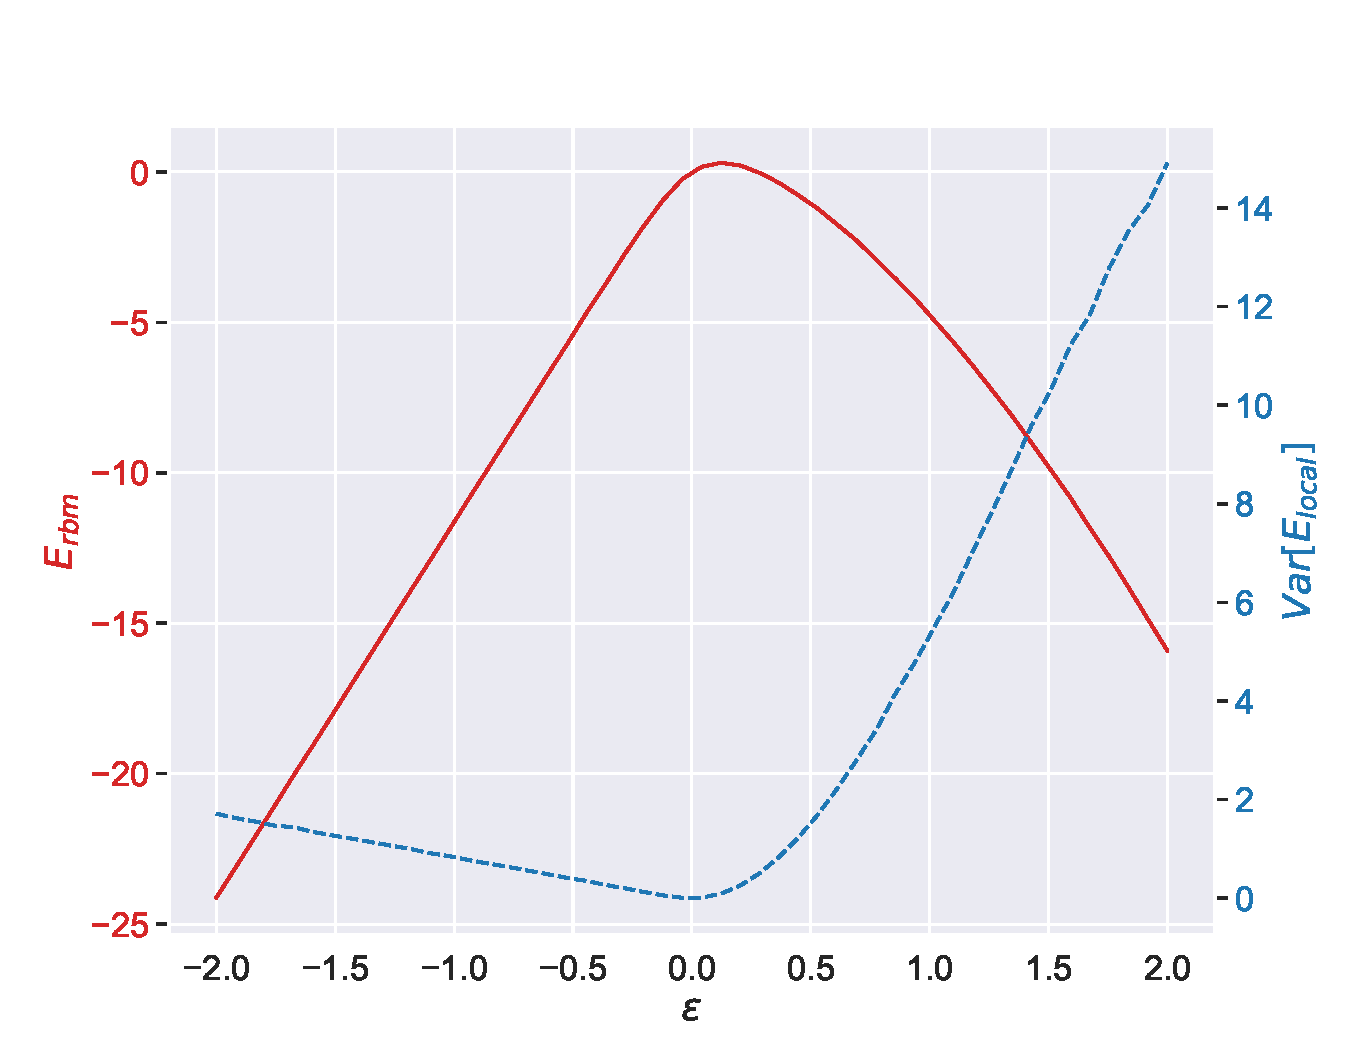
\includegraphics[width=0.95\textwidth]{Figures/Plots/Lipkin/[eps][-2.0-2.0][e=250][n=25][V=0][W=0].pdf}
  \end{center}
  \caption{The RBM prediction of the ground state energy for the Lipkin system with $V=0$ and $W=0$ with $25$ particles.}
\end{figure}

And here it would be logical for the RBM to get an even greater benefit from the fact that the true wavefunction only consists of a single basis state since a diverse wavefunction could be distributed over many times more basis states than in the smaller model example, as there are $2^N$ basis states for a $N$-particle model. It would seem to be the case towards $\varepsilon = -2$, but the RBM struggle closer to $\varepsilon = 2$ only get accentuated with a higher particle count.

\vspace{\baselineskip}
\\

To see a more complete picture of the impact that $\varepsilon$ has on the RBM accuracy we would need to include interaction strength as well. We set $V=-0.5$ and $W=0.5$ and we then get:

\begin{figure}[H]
  \begin{center}
    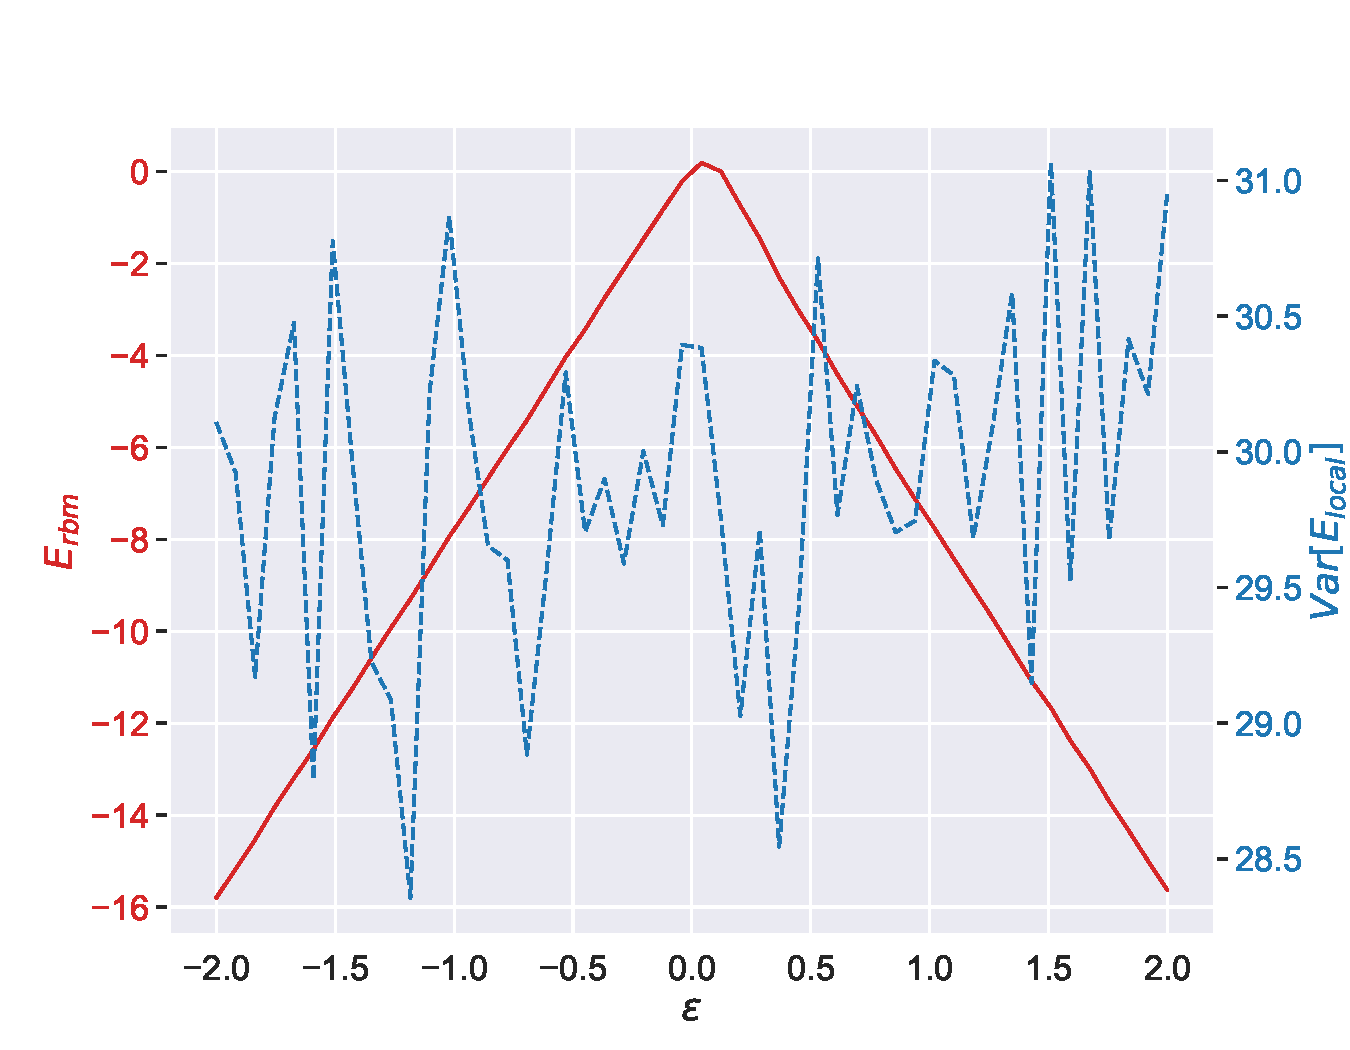
\includegraphics[width=0.95\textwidth]{Figures/Plots/Lipkin/[eps][-2.0-2.0][e=850][n=16][V=-0.5][W=0.5].pdf}
  \end{center}
  \caption{The RBM prediction of the ground state energy for the Lipkin system with $V=-0.5$ and $W=0.5$ and $16$ particles.}
\end{figure}

The variance clearly becomes more unstable as the wavefunction the machine converges to becomes more diverse. If we look at the variance axis we can see that the change in variance is not that large compared to the change in the ground state energy. As we introduce more states to the true wavefunction we see that the change in $\varepsilon$ loses its previous effect, as the it contains a wider distribution of basis states anyway.

\subsection{The effect of \texorpdfstring{$V$}{V} on RBM prediction accuracy}
Looking at the pair excitation strength we set $\varepsilon = -2$ instead, and we get:

\begin{figure}[H]
  \begin{center}
    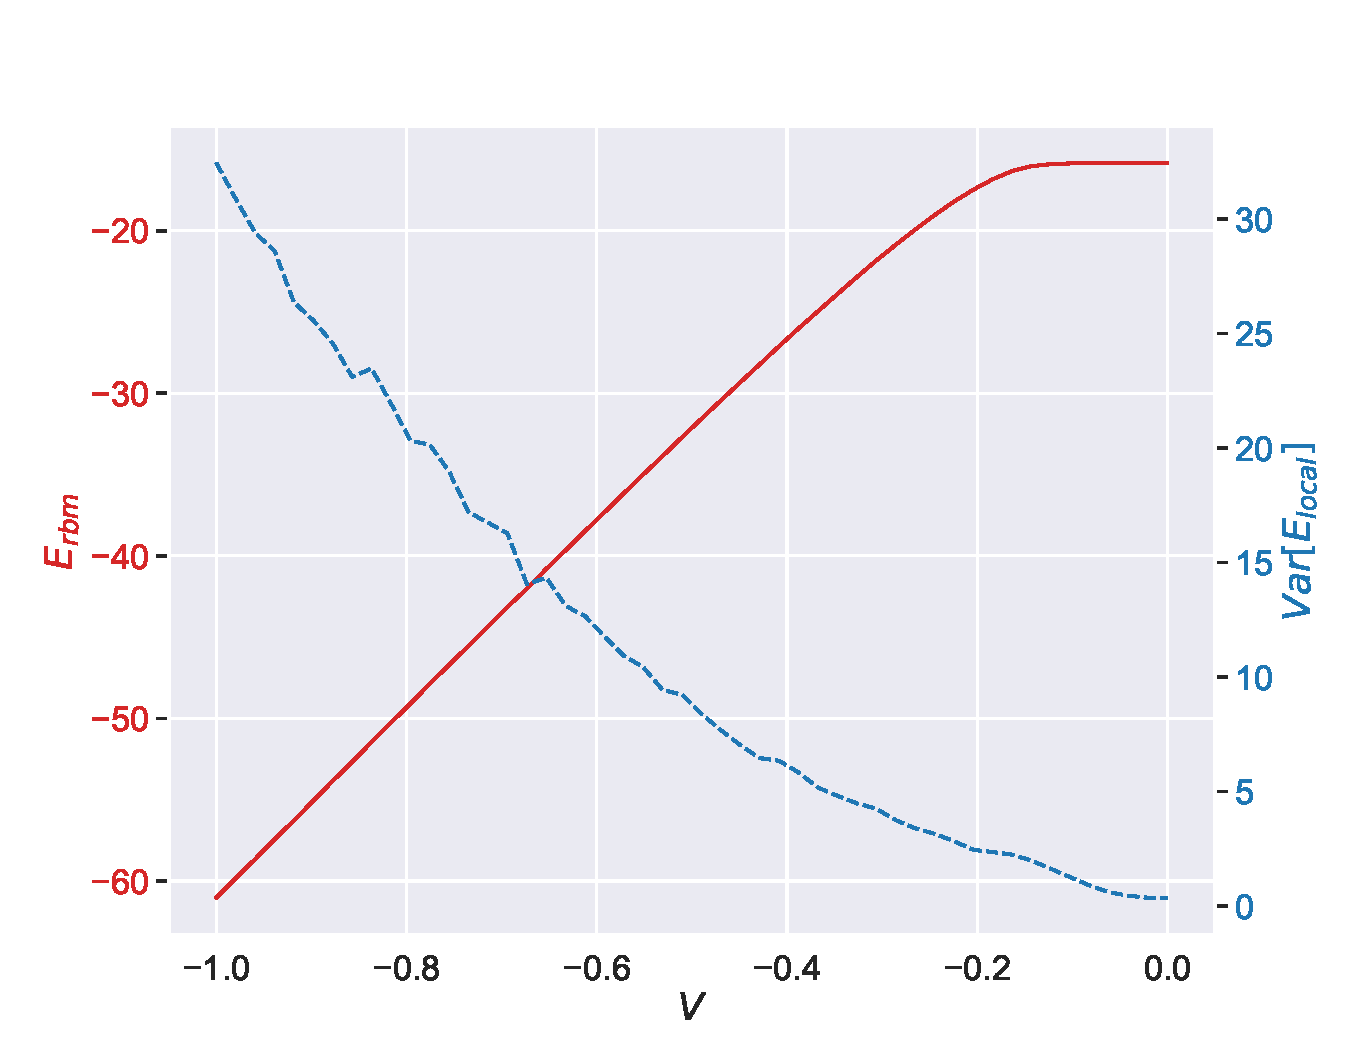
\includegraphics[width=0.95\textwidth]{Figures/Plots/Lipkin/[V][-1.0-0.0][e=850][n=16][eps=-2][W=0].pdf}
  \end{center}
  \caption{The RBM prediction of the ground state energy for the Lipkin system with $\varepsilon=-2$ and $W=0$ and $16$ particles.}
\end{figure}

Increasing the interaction strength increases the contribution of basis states one-pair-away from each other. For the RBM this would mean that for a $V$ that closes in on zero we would approach the non-interactive case, but it is also interesting that the variance decreases faster than the absolute value of the energy decreases, which tells us that the relative accuracy of the RBM gets better when it is closer to a single-basis-state true wavefunction as well.

Introducing the spin exchange interaction as well with $W=0.1$ we get the accuracy evolution:
\begin{figure}[H]
  \begin{center}
    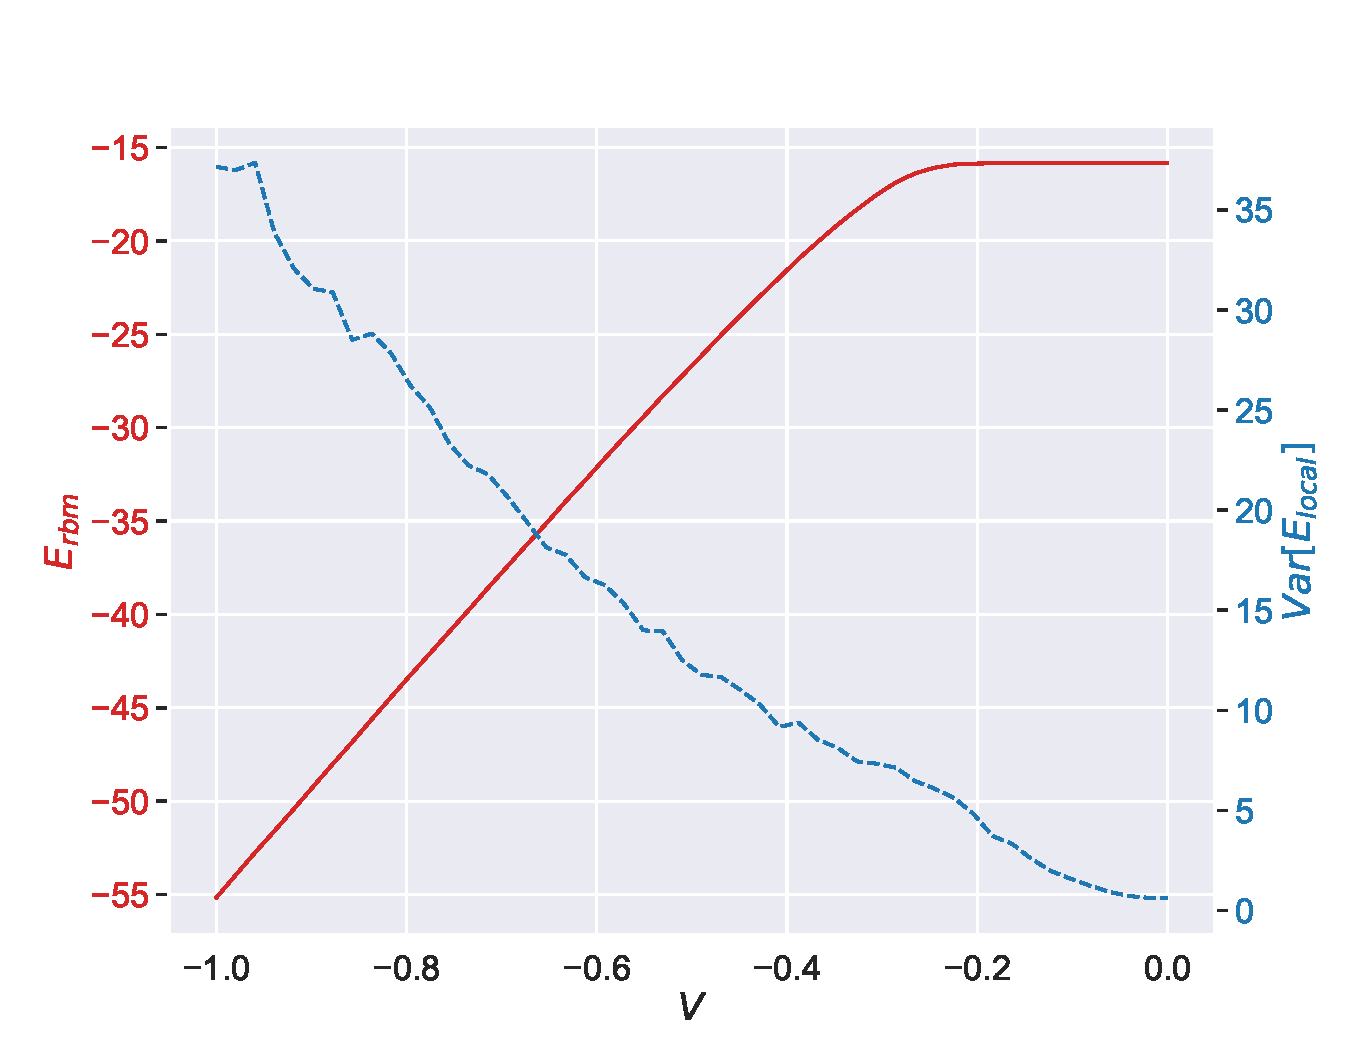
\includegraphics[width=0.95\textwidth]{Figures/Plots/Lipkin/[V][-1.0-0.0][e=850][n=16][eps=-2][W=0.1].pdf}
  \end{center}
  \caption{The RBM prediction of the ground state energy for the Lipkin system with $\varepsilon=-2$ and $W=0.1$ and $16$ particles.}
\end{figure}

Now we don't have the non-interactive case as $V$ approaches zero, but we still maintain lower variance as the interaction strength goes down, so the spin exchange does seemingly not have an effect on the accuracy.

\subsection{The effect of \texorpdfstring{$W$}{W} on RBM prediction accuracy}

We check the $W$ spin exchange interaction strength first with $V=0$, and we get:
\begin{figure}[H]
  \begin{center}
    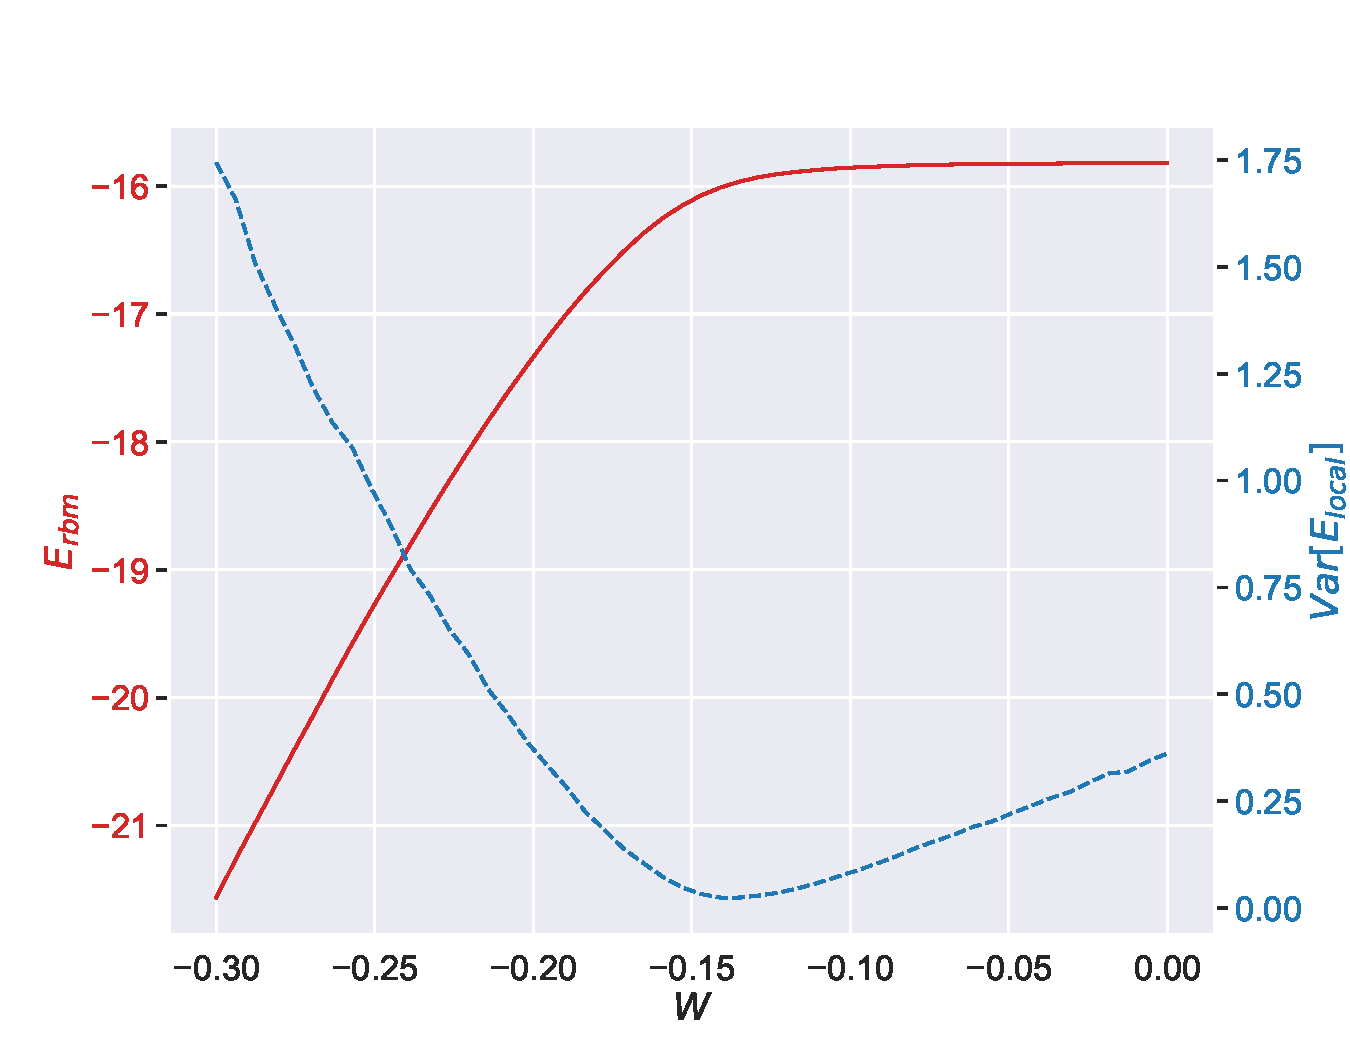
\includegraphics[width=0.95\textwidth]{Figures/Plots/Lipkin/[W][-0.3-0.0][e=850][n=16][eps=-2][V=0].pdf}
  \end{center}
  \caption{The RBM prediction of the ground state energy for the Lipkin system with $\varepsilon=-2$ and $V=0$ and $16$ particles.}
\end{figure}

First of all it is easy to see that the variance in general is ways smaller for only spin exchange. The reason for this is most likely similar to the case with only single particle energies. In the Lipkin Hamiltonian matrix the spin exchange only affect the diagonal elements. Without pair excitation we see a similar we see a similar development as that of the $V$ variable. The accuracy seem to be mainly dependent on how close the true wavefunction is to consist of a single basis state, though here it struggles more after $W \approx -0.14$. At this point the machines ground state prediction crosses $E_{rbm} = -16$, which implies the machine has converged on the single-basis-state wavefunction, lowering the variance. The variance increases again as the convergent wavefunction becomes more diverse, though it should have fallen down to $E_{rbm} = -16$ again at $W=0$.

Together with pair excitation we get that the accuracy evolves as follows:

\begin{figure}[H]
  \begin{center}
    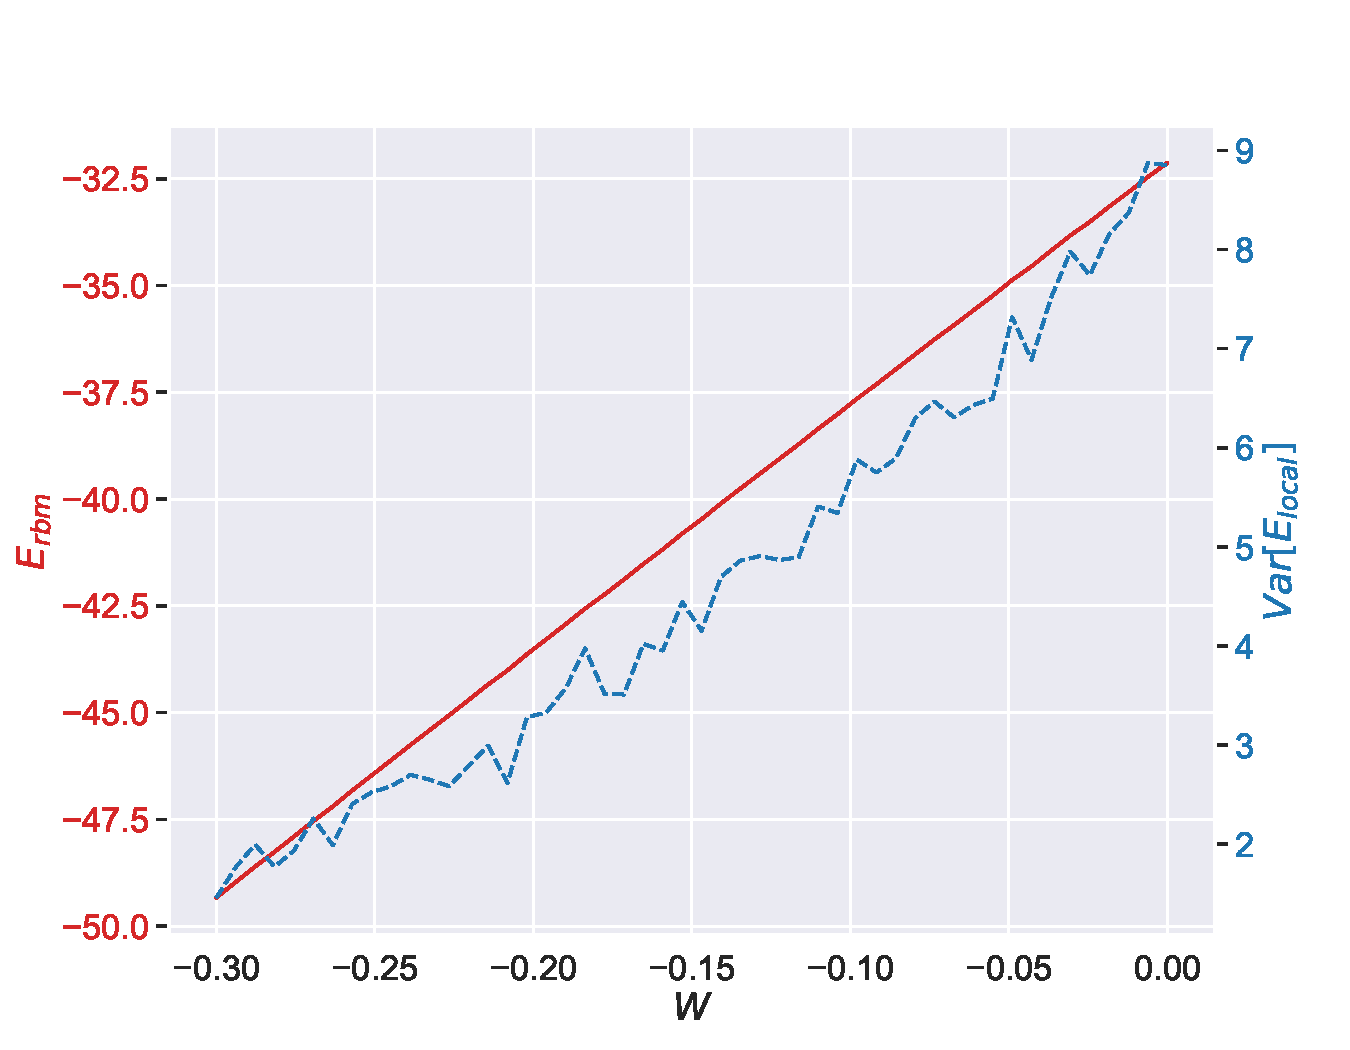
\includegraphics[width=0.95\textwidth]{Figures/Plots/Lipkin/[W][-0.3-0.0][e=850][n=16][eps=-2][V=-0.5].pdf}
  \end{center}
  \caption{The RBM prediction of the ground state energy for the Lipkin system with $\varepsilon=-2$ and $V=-0.5$ and $16$ particles.}
\end{figure}

And the variance behaves very differently. Most likely we see the effect of $W$ aligning with the lowest single particle energy state, making it even lower, and as a result making it more dominant in the ground state wavefunction. 

\subsection{System size effect on the RBM}

We plot the variance at the different system sizes for the Lipkin model with $\varepsilon =-2$, $V=-0.5$ and $W=0.1$.

\begin{figure}[H]
  \begin{center}
    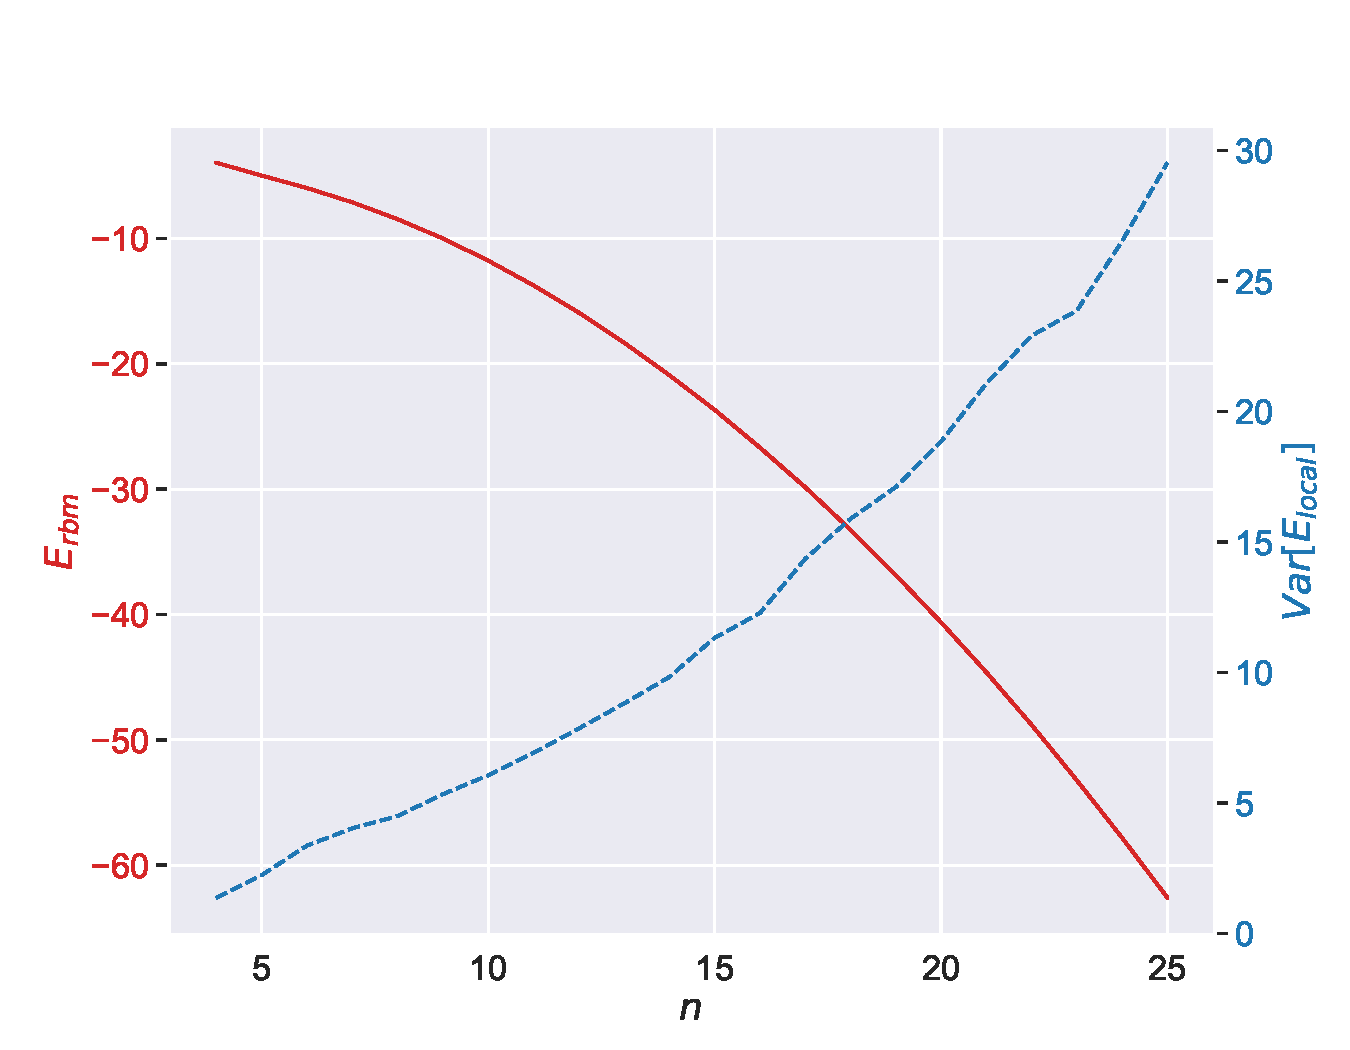
\includegraphics[width=0.95\textwidth]{Figures/Plots/Lipkin/[particles][4-25][e=850][eps=-2][V=-0.5][W=0.1].pdf}
  \end{center}
  \caption{The RBM prediction of the ground state energy for the Lipkin system with $\varepsilon=-2$ and $V=-0.5$ and $W=0.1$.}
\end{figure}

The variance overall increases as the system size goes up, but looking at the relative variance we see that that the accuracy increases as the number of particles goes up, and if we look at the RBM's relative error to the true ground state energy, we get that

\begin{figure}[H]
  \begin{center}
    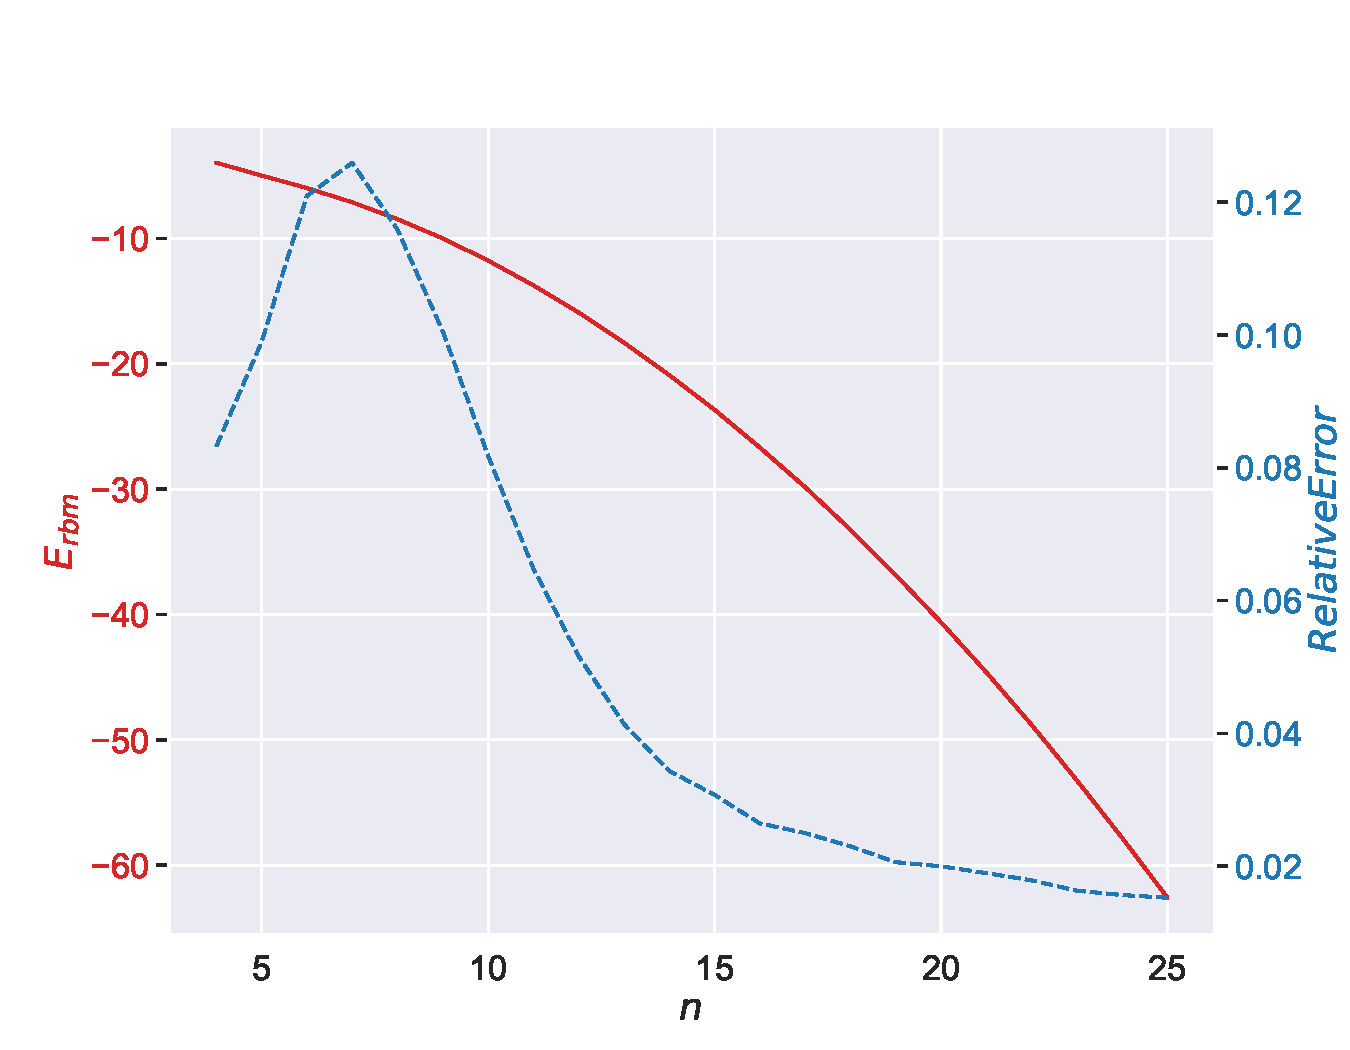
\includegraphics[width=0.95\textwidth]{Figures/Plots/Lipkin/[particles][4-25][e=850][eps=-2][V=-0.5][W=0.1]error.pdf}
  \end{center}
  \caption{The RBM prediction of the ground state energy for the Lipkin system with $\varepsilon=-2$ and $V=-0.5$ and $W=0.1$ and the relative error for different quantum system sizes.}
\end{figure}

This may seem surprising at first but the variance, and the error, of the RBM's prediction is limited by how accurate it can get the coefficients of the wavefunction, but the number of particles doesn't necessarily require a higher accuracy of the different coefficients. A higher number of particles will however increase the absolute value of the ground state energy, and as such the relative error decreases.

\subsection{Comparing computation time with diagonalization}

There are a series of factors that affects the computation time of the restricted Boltzmann machine. To make the RBM as fast as we can we will use as few epochs and Monte Carlo cycles as possible. For the computation time we also only take into account the time it takes to train the RBM and not the initialization, whose time is substantial at greater model sizes. 

\begin{figure}[H]
  \begin{center}
    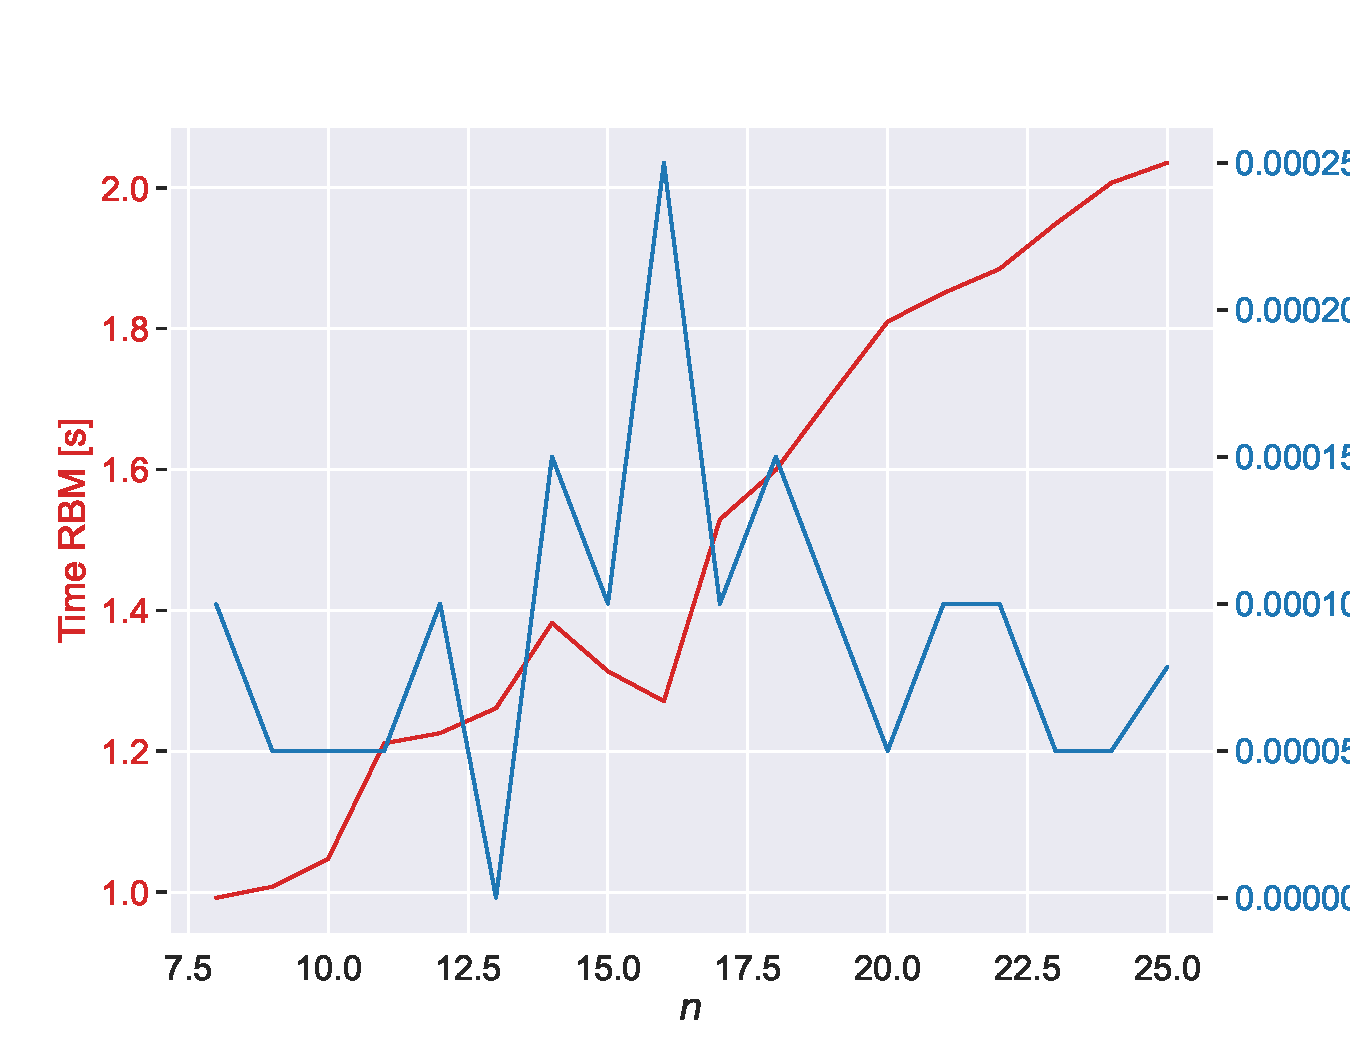
\includegraphics[width=0.8\textwidth]{Figures/Plots/Lipkin/[particles][8-25][e=500][eps=-2][V=-0.5][W=0.1]time.pdf}
  \end{center}
  \caption{The time average over twenty repeats. Here we use the Lipkin model with $\varepsilon=-2$, $V=-0.5$ and $W=0.1$.}
\end{figure}

The restricted Boltzmann machine falls short of the diagonalization method by several order of magnitude. In general the RBM has a more consistent increase in time as the system size increases, while the diagonalization time seem more uncorrelated to it. This may hint at that for diagonalization most of the time spent is used for initialization purposes. It is also possible that it detects the fact that the matrices we diagonalize are sparse, which has a more optimizes algorithm for diagonalization.




